
\section{exemple julia}

\lstset{language=julia}

{
\begin{lstlisting}
# --------------------------------------------------------------------------- 
  #Loading an instance of SPP (format: OR-library)

function loadSPP(fname)
    f=open(fname)
    # Lecture du nbre de contraintes (m) et de variables (n)
    m, n = parse.(Int, split(readline(f)) )
    # Lecture des n coefficients de la fonction economique et cree le vecteur d'entiers C
    C = parse.(Int, split(readline(f)) )
    # Lecture des m contraintes et reconstruction de la matrice binaire A
    A=zeros(Int, m, n)
    for i=1:m
        # Lecture du nombre d'elements non nuls sur la contrainte i (non utilise)
        readline(f)
        # Lecture des indices des elements non nuls sur la contrainte i
        for valeur in split(readline(f))
          j = parse(Int, valeur)
          A[i,j]=1
        end
    end
    close(f)
    return C, A
end

# --------------------------------------------------------------------------- 
# Construction gloutonne d'une solution admissible de SPP

function GreedyConstruction(C_in, A_in)

   # A completer...
   
    return x, z
end

# --------------------------------------------------------------------------- 
# Amelioration gloutonne par recherche locale d’une solution de SPP

function GreedyAmelioration(C_in, A_in, x_in, z_in)

   # A completer...
   
    return xbest, zbest
end

# --------------------------------------------------------------------------- 
# Exemple (compliant Julia v0.7 et ulterieur)

using Printf
fname = "Desktop/Data/pb_200rnd0100.dat"

C, A = loadSPP(fname)

@time x, z = GreedyConstruction(C, A)
@printf("z(xInit) = %d \n\n",z)

@time xbest, zbest = GreedyAmelioration(C, A, x, z)
@printf("z(xBest) = %d \n\n",zbest)
\end{lstlisting}
}
%
% =================================================================================
%
\section{Exemple d'exécution}

\begin{verbatim}
  0.299466 seconds (1.97 M allocations: 532.954 MiB, 11.09% gc time)
z(xInit) = 351 

  0.020743 seconds (9.12 k allocations: 70.348 MiB, 19.62% gc time)
z(xBest) = 357 
\end{verbatim}

\section{exemple d'importation de fichier jl}

\lstset{language=julia}

\begin{figure}
  \centering
  \lstinputlisting{code/RO-l3.jl}
  \caption{Projet de l'an dernier}
  \label{fig:ro-l3}
\end{figure}


\section{Contexte: les langages synchrones et \lustre, les clauses de Horn}
\label{section:background}

\subsection{Le langage \lustre}


\emph{Cette section sur \lustre est inspirée de la documentation de
  \lustre~\cite{LustreRefMan,TutorialLustre} et du rapport
  de stage de Szabolcs-Marton Bagoly~\cite{rapportstagesobi}. }
%rappels sur lustre inspirés du machin en anglais dans les anciennes versions.

\paragraph{blablabla...}
\medskip

\subsection{Nouvelle traduction de l'opérateur \texttt{Mapred/fillred}}

Le fillred est la contraction du red et du fill donc on reprend exactement la même
structure que le fill à laquelle on ajoute des tableaux en entrée. On
illustre ici pour \texttt{(res,x,y) = fillred<<test,4>>(init,a,b)}.

Comme le red, on a pour chaque variable init à gauche, un accumulateur généré
et les trois clauses suivantes :

\begin{center} $t \geq 0 \wedge State_{init}(init,a,b,res,x,y,i,t+1)
  \wedge State_a(init,a,b,res,x,y,0,t+1)\wedge State_b(init,res,x,y,a,b,0,t+1)
  \wedge Interface_{test}(init,a[0],b[0],acc[0],x[0],y[0],t+1) $

  $\implies State_{acc}(init,a,b,res,x,y,0,t)  $
\end{center}

\begin{center} $t \geq 0 \wedge State_{acc}(init,a,b,res,x,y,i-1,t)
  \wedge i > 0 \wedge i<size
  \wedge State_a(init,a,b,res,x,y,i,t+1)\wedge State_b(init,a,b,res,x,y,i,t+1)
  \wedge Interface_{test}(acc[i-1],a[i],b[i],acc[i],x[i],y[i],t+1) $

   $\implies State_{acc}(init,a,b,res,x,y,i,t) $
\end{center}

\begin{center} $t \geq 0 \wedge State_{acc}(init,a,b,res,x,y,size-1,t)
  \implies State_{res}(init,a,b,res,x,y,i,t+1) \wedge res[t] = acc[size-1][t] $
\end{center}

Avec ceci, nous avons calculé les (valeurs des cases des) tableaux mais nous ne les avons pas rendu accessibles.
Pour y remédier, on ajoute la clause suivante pour chaque tableau~:

$t \geq 0 \wedge State_{res}(init,a,b,res,x,y,i,t+1)
\implies State_x(init,a,b,res,x,y,i,t+1) $

(et idem avec $State_{y}(init,a,b,res,x,y,i,t)$)


 \begin{figure}[t!]
    \begin{subfigure}[t]{0.25\textwidth}
  \centering
  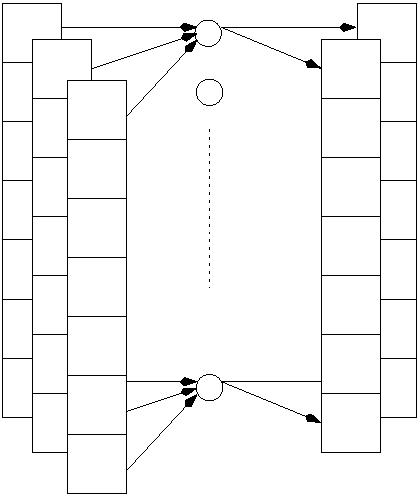
\includegraphics[scale=0.45]{fig/map.pdf}
  \caption{map}
  \label{fig:map}
    \end{subfigure}%
    ~ 
    \begin{subfigure}[t]{0.22\textwidth}
  \centering
  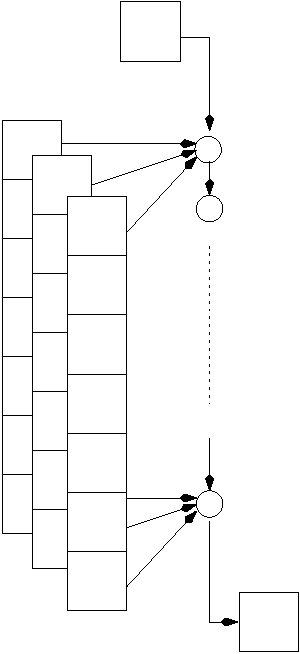
\includegraphics[scale=0.45]{fig/red.pdf}
  \caption{red}
  \label{fig:red}
\end{subfigure}
\begin{subfigure}[t]{0.25\textwidth}
  \centering
  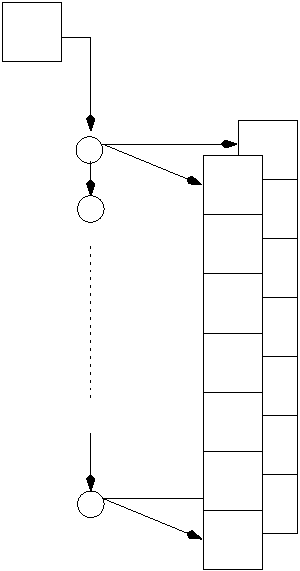
\includegraphics[scale=0.45]{fig/fill.pdf}
  \caption{fill}
  \label{fig:fill}
\end{subfigure}
\begin{subfigure}[t]{0.25\textwidth}
  \centering
  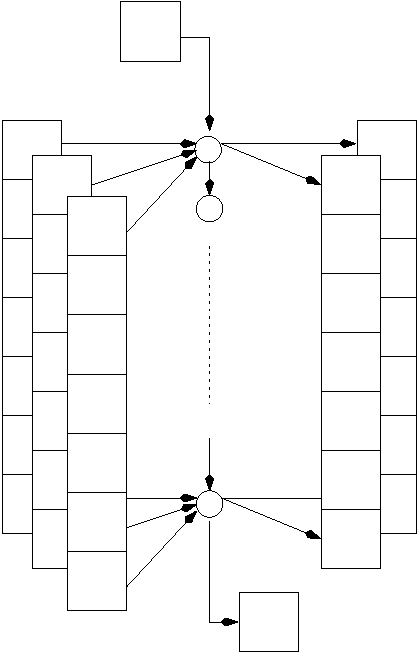
\includegraphics[scale=0.45]{fig/mapred.pdf}
  \caption{fillred}
  \label{fig:fillred}
\end{subfigure}

\caption{Illustration du comportement des itérateurs de tableaux}
\end{figure}

\paragraph{Bugs inexpliqués}
\begin{itemize}
\item unsat quand un map et un red se suivent (sat-det-max, sat-red-pos)
\item sat-bounded-interval ne termine pas
\item le fill sur un tuple non plus
\item et aucun fillred (possibilité d'une erreur dans la traduction)
\end{itemize}

\section{Conclusion}
\label{section:conclusion}

Ce travail porte donc sur
